%Results
\subsection{Experimental Infrastructure}
Figure~\ref{fig:experimental-setup} shows the infrastructure setup we used to carry out our evaluations.
We used DRAMSim2~\cite{DRAMsim2}, a cycle accurate memory simulation tool, which we customized to incorporate our refresh mechanisms. 
The input traces to DRAMSim2 were generated using the Xilinx Vivado~\cite{vivado} environment in the following manner.
The different accelerators, namely saliency, object recognitoin and action recognition, were implemented in Verilog and their output was used to generate parameters which was fed to a traffic generator.
This traffic generator outputted the memory trace comprising of read and write memory accesses.

\begin{figure}[ht!]
\centering
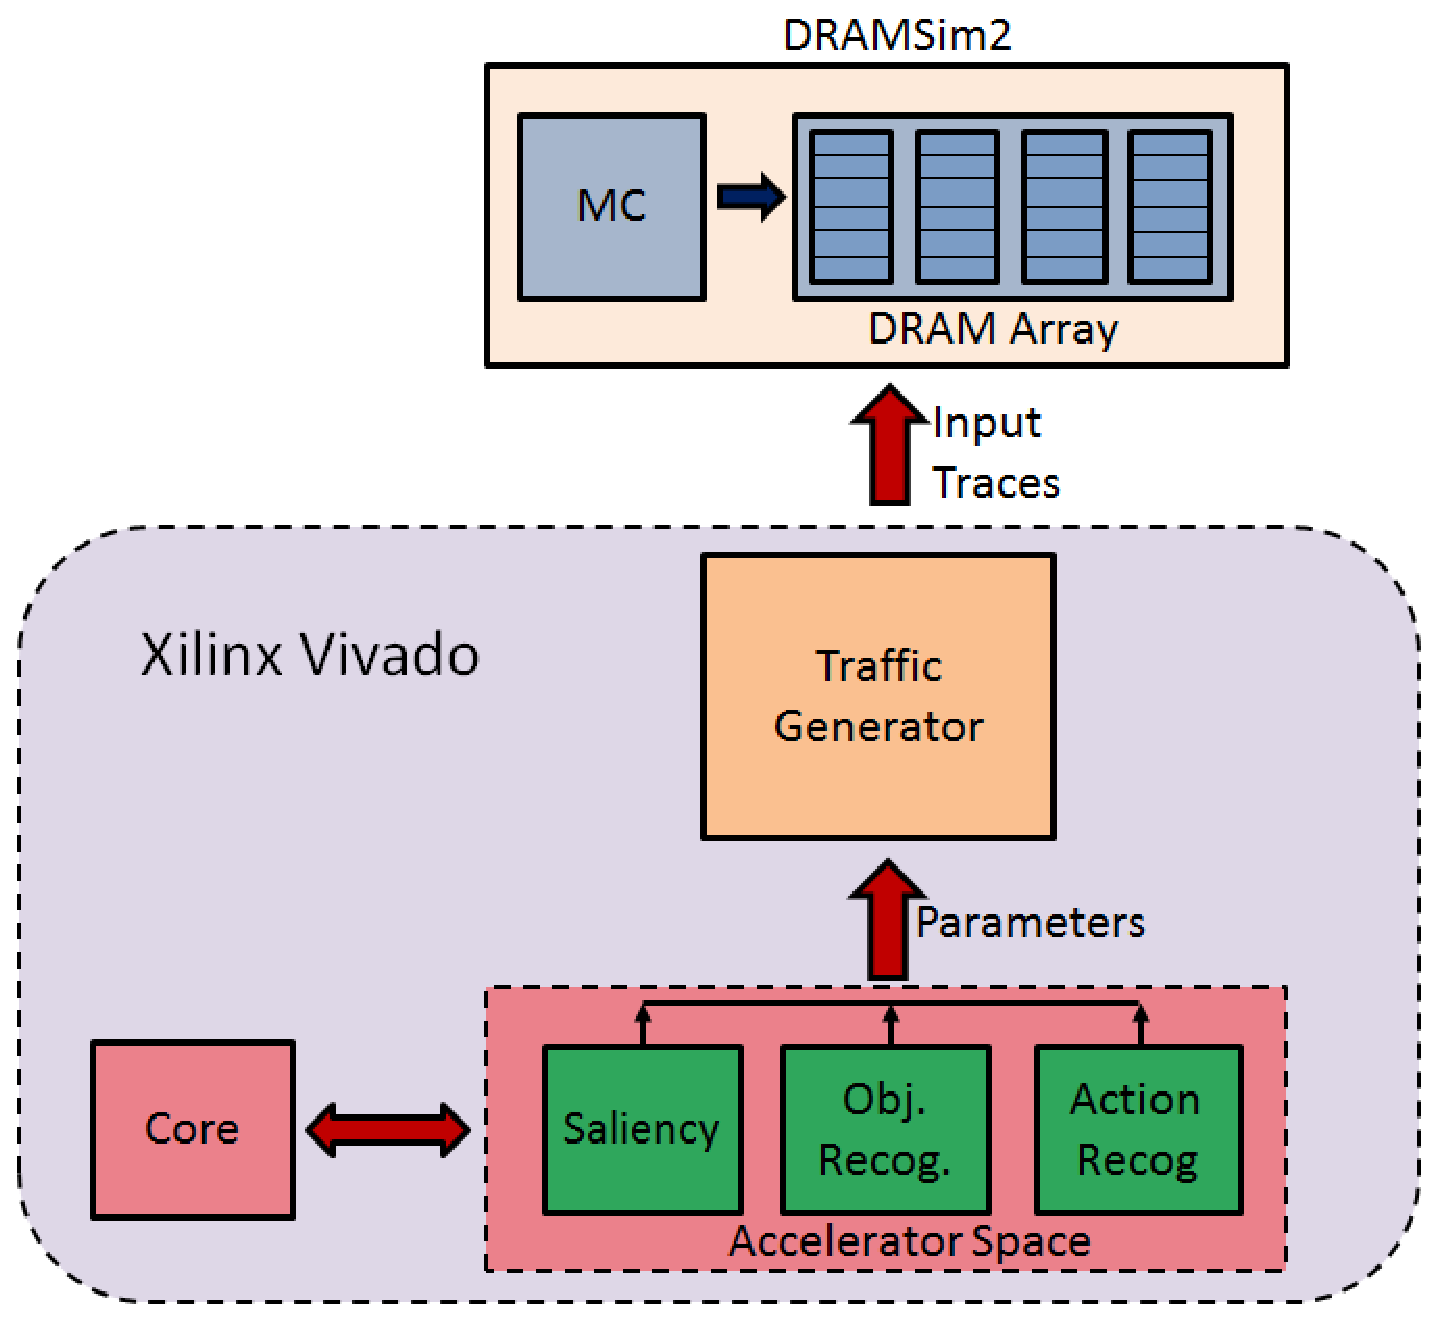
\epsfig{file=figs/experimental_setup.eps, angle=0, width=0.8\linewidth, clip=}
\caption{\label{fig:experimental-setup} Infrastructure setup}
\end{figure}

Table~\ref{tab:dram-parameters} shows the parameters used in our DRAM model, which we configured for simulation using DRAMSim2.


\begin{table}[ht!]
\footnotesize
\centering
%\vspace{-0.2cm}
\begin{tabular}{|c|c|} \hline
DRAM row & Open page\\
buffer policy & Closed after 4 accesses\\\hline
DRAM & DDR3-1600, 8 Gb, 1 channel,\\
configuration &  1 rank, 8 banks/rank \\\hline
Timing & $t_{RP}=11$, $t_{RCD}=11$\\
parameters (ns) & $t_{RFC}=350$, $t_{REFI}=7800$ \\\hline
Current & $I_{DD0}=110$, $I_{DD1}=135$, $I_{DD2P}=40=I_{DD2Q}$ \\ 
parameters (mA) & $I_{DD2N}=42$, $I_{DD3N}=45$, $I_{DD4W}=280$ \\ 
&$I_{DD4N}=270$, $I_{DD5}=215$, $I_{DD6}=12$ \\\hline
\end{tabular}
\vspace{0.1in}
\caption {DRAM parameters}
\label{tab:dram-parameters}
\end{table}

\subsection{Results}
Figure~\ref{fig:PowerResults} illustrates the total power consumption evaluated by feeding the traces generated from Vivado into DRAMSim2 for a 8 Gb based DRAM. We evaluate our scheme versus our best attempt at modeling Flikker in the given simulator. It should be noted here that when an action recognition task is triggered, a Flikker mechanism would require additional writes to move the RoIs from Non-Critical to Critical section since the action recognition would entail a 2 second video segment computation. REVA on the other hand would be dynamically capable of changing the refresh value in the RAT, thus avoiding additional writes. We also show results when we turn refresh completely off. 

\begin{figure}[ht!]
\centering
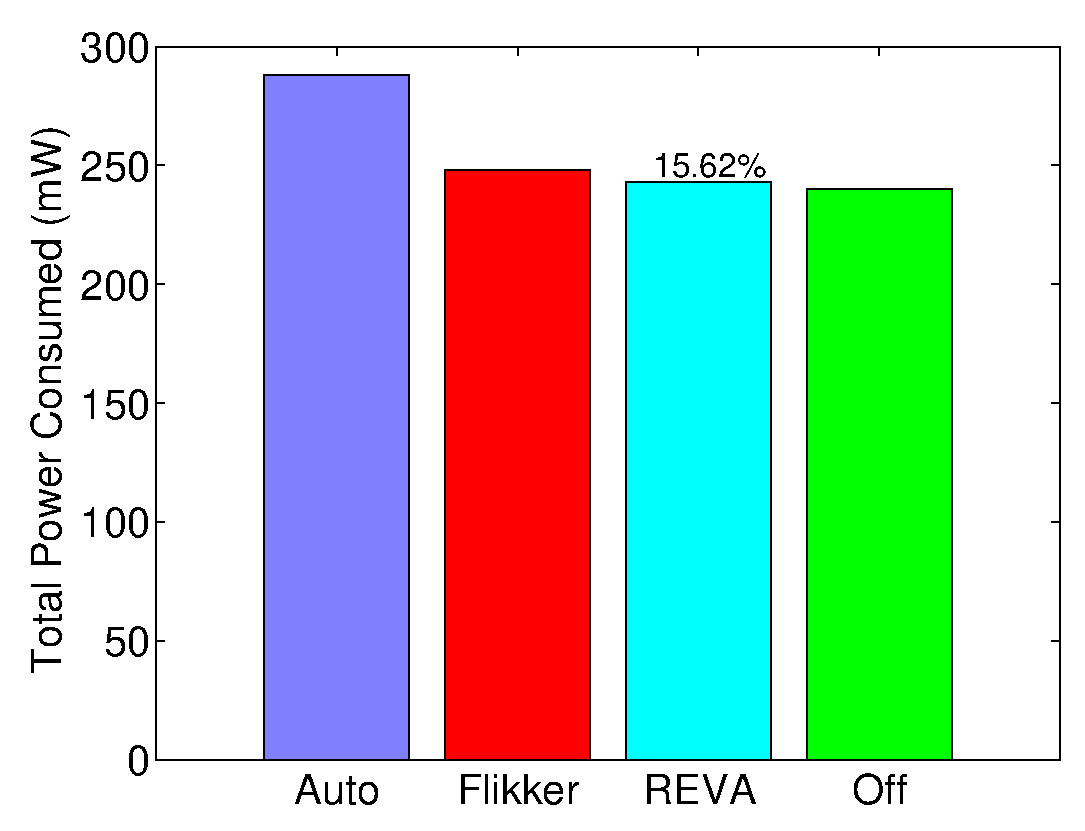
\epsfig{file=figs/DRAMPower_Improvement_8GB.eps, angle=0, width=0.9\linewidth, clip=}
\caption{\label{fig:PowerResults} Power comparisons for different schemes.}
\end{figure}

\subsection{Sensitivity Analysis}
While it can be argued that in a purely streaming embedded system, one can completely turn off refresh, we provide a compelling reason to have a variable dynamic refresh mechanism in place. There can be instances when a burst of RoIs are generated and the object recognition accelerator cannot sustain a high throughput of generating class labels. RoIs need to be buffered in the DRAM for processing at a later stage. Similarly, an object classified by HMAX may need to be evaluated further by SIFT for object matching or sub-class recognition. Then too the object needs to be stored for a period longer than the regular DRAM refresh interval. Lastly in a multi-object scenario, if a person's action is being recognized, another classified person's actions need to be buffered so as to process at a later stage. As shown in Figure~\ref{fig:ActionRecognition}, we evaluated different configurations of action recognition on the Weizmann dataset~\cite{Weizmann}. The results indicate that a purely streaming (no overlap of video segments) configuration affects accuracy considerably (by approximately 10 \%).  

\begin{figure}[ht!]
\centering
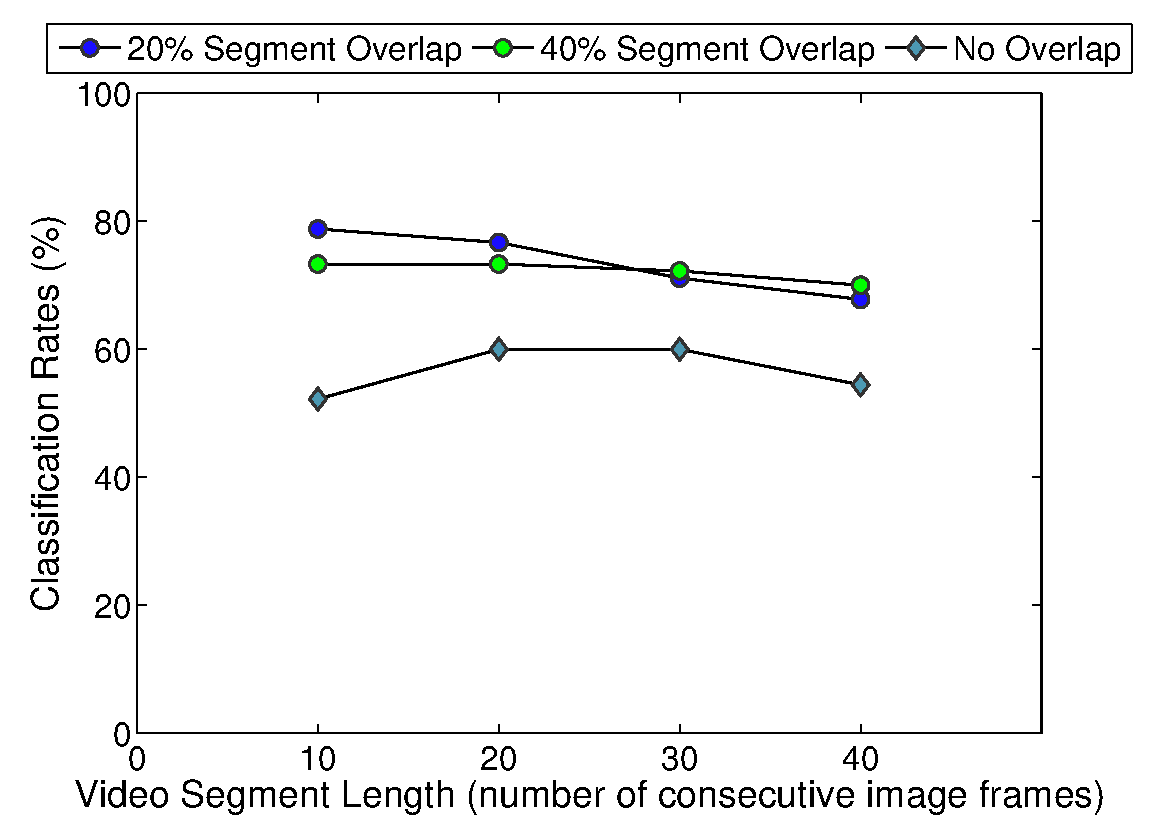
\epsfig{file=figs/ActionRecognitionAnalysis.eps, angle=0, width=0.9\linewidth, clip=}
\caption{\label{fig:ActionRecognition} Accuracy results for different configurations of video segment length and fraction of overlap between segments.}
\end{figure}


